% Options for packages loaded elsewhere
\PassOptionsToPackage{unicode}{hyperref}
\PassOptionsToPackage{hyphens}{url}
\PassOptionsToPackage{dvipsnames,svgnames,x11names}{xcolor}
%
\documentclass[
  letterpaper,
  DIV=11,
  numbers=noendperiod]{scrreprt}

\usepackage{amsmath,amssymb}
\usepackage{iftex}
\ifPDFTeX
  \usepackage[T1]{fontenc}
  \usepackage[utf8]{inputenc}
  \usepackage{textcomp} % provide euro and other symbols
\else % if luatex or xetex
  \usepackage{unicode-math}
  \defaultfontfeatures{Scale=MatchLowercase}
  \defaultfontfeatures[\rmfamily]{Ligatures=TeX,Scale=1}
\fi
\usepackage{lmodern}
\ifPDFTeX\else  
    % xetex/luatex font selection
\fi
% Use upquote if available, for straight quotes in verbatim environments
\IfFileExists{upquote.sty}{\usepackage{upquote}}{}
\IfFileExists{microtype.sty}{% use microtype if available
  \usepackage[]{microtype}
  \UseMicrotypeSet[protrusion]{basicmath} % disable protrusion for tt fonts
}{}
\makeatletter
\@ifundefined{KOMAClassName}{% if non-KOMA class
  \IfFileExists{parskip.sty}{%
    \usepackage{parskip}
  }{% else
    \setlength{\parindent}{0pt}
    \setlength{\parskip}{6pt plus 2pt minus 1pt}}
}{% if KOMA class
  \KOMAoptions{parskip=half}}
\makeatother
\usepackage{xcolor}
\setlength{\emergencystretch}{3em} % prevent overfull lines
\setcounter{secnumdepth}{5}
% Make \paragraph and \subparagraph free-standing
\makeatletter
\ifx\paragraph\undefined\else
  \let\oldparagraph\paragraph
  \renewcommand{\paragraph}{
    \@ifstar
      \xxxParagraphStar
      \xxxParagraphNoStar
  }
  \newcommand{\xxxParagraphStar}[1]{\oldparagraph*{#1}\mbox{}}
  \newcommand{\xxxParagraphNoStar}[1]{\oldparagraph{#1}\mbox{}}
\fi
\ifx\subparagraph\undefined\else
  \let\oldsubparagraph\subparagraph
  \renewcommand{\subparagraph}{
    \@ifstar
      \xxxSubParagraphStar
      \xxxSubParagraphNoStar
  }
  \newcommand{\xxxSubParagraphStar}[1]{\oldsubparagraph*{#1}\mbox{}}
  \newcommand{\xxxSubParagraphNoStar}[1]{\oldsubparagraph{#1}\mbox{}}
\fi
\makeatother

\usepackage{color}
\usepackage{fancyvrb}
\newcommand{\VerbBar}{|}
\newcommand{\VERB}{\Verb[commandchars=\\\{\}]}
\DefineVerbatimEnvironment{Highlighting}{Verbatim}{commandchars=\\\{\}}
% Add ',fontsize=\small' for more characters per line
\usepackage{framed}
\definecolor{shadecolor}{RGB}{241,243,245}
\newenvironment{Shaded}{\begin{snugshade}}{\end{snugshade}}
\newcommand{\AlertTok}[1]{\textcolor[rgb]{0.68,0.00,0.00}{#1}}
\newcommand{\AnnotationTok}[1]{\textcolor[rgb]{0.37,0.37,0.37}{#1}}
\newcommand{\AttributeTok}[1]{\textcolor[rgb]{0.40,0.45,0.13}{#1}}
\newcommand{\BaseNTok}[1]{\textcolor[rgb]{0.68,0.00,0.00}{#1}}
\newcommand{\BuiltInTok}[1]{\textcolor[rgb]{0.00,0.23,0.31}{#1}}
\newcommand{\CharTok}[1]{\textcolor[rgb]{0.13,0.47,0.30}{#1}}
\newcommand{\CommentTok}[1]{\textcolor[rgb]{0.37,0.37,0.37}{#1}}
\newcommand{\CommentVarTok}[1]{\textcolor[rgb]{0.37,0.37,0.37}{\textit{#1}}}
\newcommand{\ConstantTok}[1]{\textcolor[rgb]{0.56,0.35,0.01}{#1}}
\newcommand{\ControlFlowTok}[1]{\textcolor[rgb]{0.00,0.23,0.31}{\textbf{#1}}}
\newcommand{\DataTypeTok}[1]{\textcolor[rgb]{0.68,0.00,0.00}{#1}}
\newcommand{\DecValTok}[1]{\textcolor[rgb]{0.68,0.00,0.00}{#1}}
\newcommand{\DocumentationTok}[1]{\textcolor[rgb]{0.37,0.37,0.37}{\textit{#1}}}
\newcommand{\ErrorTok}[1]{\textcolor[rgb]{0.68,0.00,0.00}{#1}}
\newcommand{\ExtensionTok}[1]{\textcolor[rgb]{0.00,0.23,0.31}{#1}}
\newcommand{\FloatTok}[1]{\textcolor[rgb]{0.68,0.00,0.00}{#1}}
\newcommand{\FunctionTok}[1]{\textcolor[rgb]{0.28,0.35,0.67}{#1}}
\newcommand{\ImportTok}[1]{\textcolor[rgb]{0.00,0.46,0.62}{#1}}
\newcommand{\InformationTok}[1]{\textcolor[rgb]{0.37,0.37,0.37}{#1}}
\newcommand{\KeywordTok}[1]{\textcolor[rgb]{0.00,0.23,0.31}{\textbf{#1}}}
\newcommand{\NormalTok}[1]{\textcolor[rgb]{0.00,0.23,0.31}{#1}}
\newcommand{\OperatorTok}[1]{\textcolor[rgb]{0.37,0.37,0.37}{#1}}
\newcommand{\OtherTok}[1]{\textcolor[rgb]{0.00,0.23,0.31}{#1}}
\newcommand{\PreprocessorTok}[1]{\textcolor[rgb]{0.68,0.00,0.00}{#1}}
\newcommand{\RegionMarkerTok}[1]{\textcolor[rgb]{0.00,0.23,0.31}{#1}}
\newcommand{\SpecialCharTok}[1]{\textcolor[rgb]{0.37,0.37,0.37}{#1}}
\newcommand{\SpecialStringTok}[1]{\textcolor[rgb]{0.13,0.47,0.30}{#1}}
\newcommand{\StringTok}[1]{\textcolor[rgb]{0.13,0.47,0.30}{#1}}
\newcommand{\VariableTok}[1]{\textcolor[rgb]{0.07,0.07,0.07}{#1}}
\newcommand{\VerbatimStringTok}[1]{\textcolor[rgb]{0.13,0.47,0.30}{#1}}
\newcommand{\WarningTok}[1]{\textcolor[rgb]{0.37,0.37,0.37}{\textit{#1}}}

\providecommand{\tightlist}{%
  \setlength{\itemsep}{0pt}\setlength{\parskip}{0pt}}\usepackage{longtable,booktabs,array}
\usepackage{calc} % for calculating minipage widths
% Correct order of tables after \paragraph or \subparagraph
\usepackage{etoolbox}
\makeatletter
\patchcmd\longtable{\par}{\if@noskipsec\mbox{}\fi\par}{}{}
\makeatother
% Allow footnotes in longtable head/foot
\IfFileExists{footnotehyper.sty}{\usepackage{footnotehyper}}{\usepackage{footnote}}
\makesavenoteenv{longtable}
\usepackage{graphicx}
\makeatletter
\def\maxwidth{\ifdim\Gin@nat@width>\linewidth\linewidth\else\Gin@nat@width\fi}
\def\maxheight{\ifdim\Gin@nat@height>\textheight\textheight\else\Gin@nat@height\fi}
\makeatother
% Scale images if necessary, so that they will not overflow the page
% margins by default, and it is still possible to overwrite the defaults
% using explicit options in \includegraphics[width, height, ...]{}
\setkeys{Gin}{width=\maxwidth,height=\maxheight,keepaspectratio}
% Set default figure placement to htbp
\makeatletter
\def\fps@figure{htbp}
\makeatother

\KOMAoption{captions}{tableheading}
\makeatletter
\@ifpackageloaded{bookmark}{}{\usepackage{bookmark}}
\makeatother
\makeatletter
\@ifpackageloaded{caption}{}{\usepackage{caption}}
\AtBeginDocument{%
\ifdefined\contentsname
  \renewcommand*\contentsname{Table of contents}
\else
  \newcommand\contentsname{Table of contents}
\fi
\ifdefined\listfigurename
  \renewcommand*\listfigurename{List of Figures}
\else
  \newcommand\listfigurename{List of Figures}
\fi
\ifdefined\listtablename
  \renewcommand*\listtablename{List of Tables}
\else
  \newcommand\listtablename{List of Tables}
\fi
\ifdefined\figurename
  \renewcommand*\figurename{Figure}
\else
  \newcommand\figurename{Figure}
\fi
\ifdefined\tablename
  \renewcommand*\tablename{Table}
\else
  \newcommand\tablename{Table}
\fi
}
\@ifpackageloaded{float}{}{\usepackage{float}}
\floatstyle{ruled}
\@ifundefined{c@chapter}{\newfloat{codelisting}{h}{lop}}{\newfloat{codelisting}{h}{lop}[chapter]}
\floatname{codelisting}{Listing}
\newcommand*\listoflistings{\listof{codelisting}{List of Listings}}
\makeatother
\makeatletter
\makeatother
\makeatletter
\@ifpackageloaded{caption}{}{\usepackage{caption}}
\@ifpackageloaded{subcaption}{}{\usepackage{subcaption}}
\makeatother

\ifLuaTeX
  \usepackage{selnolig}  % disable illegal ligatures
\fi
\usepackage{bookmark}

\IfFileExists{xurl.sty}{\usepackage{xurl}}{} % add URL line breaks if available
\urlstyle{same} % disable monospaced font for URLs
\hypersetup{
  pdftitle={Transboundary coastal waterbird trends in the Salish Sea},
  pdfauthor={Danielle Ethier},
  colorlinks=true,
  linkcolor={blue},
  filecolor={Maroon},
  citecolor={Blue},
  urlcolor={Blue},
  pdfcreator={LaTeX via pandoc}}


\title{Transboundary coastal waterbird trends in the Salish Sea}
\author{Danielle Ethier}
\date{2025-06-01}

\begin{document}
\maketitle

\renewcommand*\contentsname{Table of contents}
{
\hypersetup{linkcolor=}
\setcounter{tocdepth}{2}
\tableofcontents
}

\bookmarksetup{startatroot}

\chapter{Welcome Data Users!}\label{welcome-data-users}

\section{Goals}\label{0.1Intro}

The goals of this user guide is to empower resource managers to leverage
standardized citizen-science monitoring data, collected by the British
Columbia Coastal Waterbird Survey (BCCWS) and Puget Sound Seabird Survey
(PSSS), to (1) obtain scientifically credible measures of abundance
trends of coastal waterbirds in the transboundary waters of the Salish
Seas at scales appropriate for resource management, (2) identify
priority species for conservation, and (3) provide resource managers
with openly accessible annual indices of abundance for model-based
management planning. In turn, these modelling outputs can be used to
assess environmental and human-induced mechanisms of waterbird changes
and provide a foundation from which to tease apart whether local
population fluctuations are a result of true changing abundance or
shifts in species distributions over time.

Data users are encourage to review the
\href{https://birdscanada.github.io/TransboundaryData_SalishSea/}{Transboundary
avian data for the Salish Sea} user guide, which details addition avian
datasets and spatial data layers available for the Salish Sea.

\section{Using this Technical Guide}\label{0.2Intro}

This guide provides users with step-by-step instructions and user
defined parameters to customize the analysis. The workflow is as
follows:

\textbf{Chapter 1: Overview of Methods}

The methods section is technical, but users are strongly encouraged to
read this section in full before proceeding with an analysis.

\textbf{Chapter 2: Data Access and Cleaning}

Data cleaning and formatting steps are largely done in the background
and were vetted by the BCCWS and PSSS program coordinators. Species
selected for the analysis are those which the program coordinators felt
were representative and regularly monitored by both survey protocols.

\href{Data/GuildList.csv}{GuildList.csv} can be modified by data users
if species are missing or modification are deemed needed.

Sampling events plot should be inspected prior to proceeding with the
analysis.

\textbf{Chapter 3: Analysis and Visualization}

Several user defined options are presented here to customize the
analysis

Users Select to following parameter settings (or can use the defaults):

\begin{itemize}
\item
  \texttt{Y1} = Start year of analysis
\item
  \texttt{Y2} = End year of analysis
\item
  \texttt{model} = Specify the model as iCAR (discrete space) or SPDE
  (continuous space)

  \begin{itemize}
  \item
    if \texttt{model} = ``iCAR'' the user will need to load a
    multi-polygon shapefile or use the default provided

    \begin{itemize}
    \item
      Option is given to assign data point to polygons they fall
      \texttt{within} or are \texttt{nearest}
    \item
      Option is given to assign weights to areas for full study area
      trend roll up.
    \end{itemize}
  \item
    if \texttt{model} = ``SPDE'' the user can select the \texttt{area}
    as SALISHSEA, BCCWS, or PSSS
  \end{itemize}
\item
  \texttt{species.list} can either be all the species the programs have
  in common, or the user can select species of interest
\item
  \texttt{guild} can be turned to ``yes'' to indicate the user wishes to
  do a guild level analysis. Default this is set to ``no''.

  \begin{itemize}
  \tightlist
  \item
    if \texttt{guild} = ``yes'' the user can selece the \texttt{type} as
    family, diet, or migration.
  \end{itemize}
\item
  Minimum data requirement setting include: \texttt{min.abundance},
  \texttt{min.year}, and \texttt{nsites}
\item
  Model specifications include the distributional family \texttt{fam},
  and the random and sptail priors \texttt{hyper.idd},
  \texttt{prior.range}, \texttt{prior.sigma}
\item
  A meaningful \texttt{name} is given to the output files - When
  displaying results, users can select between the ``endpoint'' or
  ``slope'' \texttt{trend}
\end{itemize}

This guide assumes that you have a basic understanding of R. All the R
scripts and data resources associated with this project are available on
the \href{https://github.com/BirdsCanada/SalishSeaTrends}{Birds Canada
GitHub} page and in the \hyperref[9.9BirdsCan]{Resource} section of this
guide. If you run into issues executing the code or it generates errors,
please open a git issue, or send an email to dethier@birdscanada.org.

\section{Acknowledgement}\label{0.3Intro}

This project was financially supported by the SeaDoc Society, a program
of the Karen C. Drayer Wildlife Health Center, School of Veterinary
Medicine, University of California, Davis.

\bookmarksetup{startatroot}

\chapter{Project Overview}\label{project-overview}

\section{Background}\label{1.1Intro}

Waterbird species that overwinter in the Salish Sea have experienced
significant changes in abundance in recent decades, the causes of which
remain largely unresolved. Globally significant populations of sea
ducks, including several vital sign indicators, are among the species
experiencing declines. Long-term standardized monitoring programs have
demonstrated their value for assessing broad-scale population trends of
many coastal waterbirds in parts of the Salish Sea, however, a seamless
approach for generating and updating transboundary trends for species
and guilds has yet to be realized, nor has an approach for assessing
finer-scale trends at geographic extents relevant to conservation
planners been developed.

The analysis scripts developed herein closes this technical and
information gap by applying spatially explicit hierarchical analytical
techniques in a Bayesian framework to two parallel citizen science
programs in Canada (British Columbia Coastal Waterbird Survey; BCCWS)
and the U.S. (Puget Sound Seabird Survey; PSSS). Collectively, these
programs have monitored overwintering waterbirds across 476 sampling
locations in the Salish Sea since 2008 using a nearly identical
protocol. The statistical approach we deploy takes advantage of the
spatial relationships among count sites, allowing for more robust
parameter estimates in places where data are sparse, and enabling trend
outputs at finer spatial scales relevant to local management
organizations. Further, by making these results and analytical code
openly accessible, we empower resource managers with regionally
tailored, regularly updated trends and annual indices of abundance,
which will ultimately expedite our understanding of drivers of change
and provide baselines from which to assess the outcomes of our
management actions.

\section{Methods}\label{1.2Intro}

The analysis framework is spatially explicit, meaning the model borrows
strength from data-rich regions to stabilize estimates in areas with
sparse sampling. The user can choose from one of two spatially explicit
analytical approaches. Both use spatially varying coefficients (SVCs,
Gelfand et al.~2003) to account for relationships between variables (in
this case, counts of birds) that are not uniform across large spatial
areas. This modelling approach was first applied to continent wide bird
abundance data to assess winter bird population trends using discrete
aerial units (Meehan et al.~2019) and an intrinsic conditional
autoregressive model (iCAR; Besag 1974). The modelling framework was
later adapted (Meehan et al.~2024) to incorporate continuous space using
a triangulated model mesh and stochastic partial differential equation
(SPDE; Lindgren et al.~2022). The benefits of a continuous-space (SPDE)
versus a discrete-space (iCAR) models are (1) finer resolution of
trends, (2) a better understanding of the range of spatial correlation,
and (3) a reduction in boundary effects associated with discrete-space
analyses. However, many management units (such as geopolitical
boundaries) are divided by discrete polygons, making the iCAR approach
appropriate in many instances. We therefore develop workflows which
allows for both an iCAR and SPDE SCV approach to derive estimates of
annual relative abundance as well as long-term trends of coastal
waterbirds in the Salish Sea.

\hyperref[2.1Data]{Details on data collection and processing can be
found in the next section of this user guide}

The basic statistical unit for the analysis was the maximum yearly count
of each species at a survey site. We initially structured the analysis
at a monthly resolution, treating monthly counts at sites as our
response variable. However, model diagnostics revealed convergence
failures and inflated variance components indicating poor identifiable
of monthly effects. To balance temporal resolution with model stability,
we aggregated counts to the maximum yearly count at each survey site.
This aggregation reduced overdispersion while maintaining ecological
relevance.

Species must meet the minimum data requirements in order to be included
in the analysis. By default, these include (1) minimum annual abundance
\textgreater10 individuals across all sites, (2) detection in
\textgreater50\% of study years (specifically \textgreater(Y₂-Y₁)/2
years where Y₁ and Y₂ represent the study period endpoints), and (3)
presence at \textgreater10 distinct monitoring locations.
\hyperref[3.1Analysis]{Minimum data filters can be adjusted by users
before running the analysis}.

Extreme outliers in observation counts are identified using a
quantile-based threshold. We calculated the outlier cutoff as three
times the 99th percentile of the maximum observation count. This was
done to prevent disproportionate influence from rare extreme values and
to aid in model fit. Data from 2020 were also removed to due survey
disruptions caused by COVID-19.

We modeled the maximum observed counts yₐₜ at site a and year t using a
negative binomial distribution: yₐₜ ∼ NB(μₐₜ, ϕ) where μₐₜ =
exp{[}log(Dₐₜ) + fₜ + γₖ + α(sₐ){]}. The linear predictor incorporated
survey duration Dₐₜ as an offset, a temporal parameter γₖ with an
independent and identically distributed (IID) random effect to allow for
random fluctuations in counts from year to year, and a site-level random
effects fₜ with IID.

The spatial component on abundance α(sₐ) uses either the SPDE or iCAR
approach. \hyperref[3.1Analysis]{This is user defined before running the
analysis.}

The SPDE approach uses a mesh, featuring maximum edge lengths of 25 km
(inner domain) and 50 km (outer buffer), minimum vertex spacing of 2 km,
and boundary constraints derived from coastline geometry. For the
spatial range parameter, we set the prior such that there was a 50\%
probability that the spatial correlation range exceeded 20 km (i.e.,
P(range \textgreater{} 20 km) = 0.5). For the spatial standard
deviation, we set the prior so that there was a 10\% probability that
the marginal standard deviation exceeded 1 (i.e., P(σ \textgreater{} 1)
= 0.1). These priors provide weakly informative regularization,
reflecting plausible spatial scales and variation while avoiding over
fitting. \hyperref[3.1SPDE]{These priors can be adjusted by users before
running an analysis}.

The iCAR approach assigned spatially structured random intercepts for
each provided polygon based on the neighborhood adjacency (1=neighbour,
0 otherwise). This allowed for information on relative abundance to be
shared across neighbouring polygons. Values of α(sₐ) came from a normal
distribution with a mean value related to the average of adjacent cells
and with a conditional variance proportional to the variance across
adjacent cells and inversely proportional to the number of adjacent
cells. We provide an example using the ``Watersheds in the Salish Sea
Bioregion'' layer from the
\href{https://salish-sea-atlas-data-wwu.hub.arcgis.com/}{Salish Sea
Atlas Data}. Users can \hyperref[3.1Analysis]{upload a multipolygon
spatial layer}, which covers part or all of the Salish Sea to run the
analysis for the management jurisdictions of interest.

Models are fitted via integrated nested Laplace approximation (INLA)
with 1,000 posterior samples drawn for uncertainty quantification. We
computed annual abundance indices Ñₜ by summing exponentiated linear
predictos of abundances, then derived trends using the slope and enpoint
methods.

\begin{itemize}
\item
  Slope Trend = 100 x (exp(coef(lm(log(NY) \textasciitilde{} Y)){[}2{]})
  - 1)

  \emph{The average annual rate of change across all years, estimated
  via ordinary least squares regression on log-transformed predicted
  abundances. Assumes a linear trend on a log scale. This is the output
  we would encourage users to select for making assessment of trends, as
  the end-point trend will be less stable given our model structure.}
\item
  Endpoint Trend = 100 × {[}(Ñ\_Y₂/Ñ\_Y₁)\^{}\{1/(Y₂-Y₁)\} - 1{]}.

  \emph{The constant annual rate that would transition NY1 to NY2 over
  Y2−Y1 years, assuming exponential growth. This is equivalent to the
  geometric mean of annual growth rates, and is standard with the
  Canadian Breeding Bird Survey (BBS) analysis. Because the BBS uses a
  GAM year effect, the smoothing of the annual indices makes the
  end-point approach more stable as it mitigates the sensitivity of
  anomalous start/end years.}
\end{itemize}

Credible intervals reflected the 2.5\% and 97.5\% quantiles of posterior
trend estimates, with interval width calculated as their difference. The
iCAR model also produces area-weighted composite indices of abundance,
where \hyperref[3.1.1Analysis]{weights are assigned by the user as being
equal or based on the polygon area}.

For analyses conducted at the guild level, we included an additional
species-level random effect, also modeled with an IID, to account for
unstructured heterogeneity among species.

\section{Results}\label{1.3Intro}

Select model outputs (national and international trends) are accessible
through the \emph{naturecounts} R package and will be made available
through the web portal in late 2025. The outputs from this analysis will
therefore provide resource managers with openly accessible annual
indices of abundance for model-based management planning. User generated
output will be stored in the output folder in the working directory of
this project.

\bookmarksetup{startatroot}

\chapter{Data Access and Cleaning}\label{data-access-and-cleaning}

Before you get started, run the \texttt{setup.R} script to install and
load the necessary packages and functions for this analysis.

\begin{Shaded}
\begin{Highlighting}[]
\FunctionTok{source}\NormalTok{(}\StringTok{"Scripts/00\_Setup.R"}\NormalTok{)}
\end{Highlighting}
\end{Shaded}

\section{British Columbia Coastal Waterbird Survey
(BCCWS)}\label{2.1Data}

\subsection{Protocol}\label{protocol}

BCCWS data collection protocol can be found online
\href{https://www.birdscanada.org/bird-science/british-columbia-coastal-waterbird-survey/bccws_resources}{here}.

In short, surveys have been conducted by volunteers using a standardized
protocol and data collection
\href{https://birdscanada.b-cdn.net/wp-content/uploads/2021/02/BCCWS_Datasheet.pdf}{sheets}.
Shore-based counts are completed monthly on or near the second Sunday of
each month from September to April. Surveys are complete within
approximately 2 hours of high tide to maximize the opportunity for close
observation. All waterbirds observed to a distance of 1 km from the high
tide line are counted, except those that fly through without stopping.
In the case of larger flocks, numbers are estimated by counting
individuals and species in groups and scaling up (see
\href{https://birdscanada.b-cdn.net/wp-content/uploads/2020/02/BCCWS-Training-Module.pdf}{Training
Module for Volunteers}). Data are entered through a customized online
data entry system available on the Birds Canada website,
\href{https://birdscanada.github.io/www.birdscanada.\%20org/birdmon/default/main.jsp}{NatureCounts}.
Observations are processed using the eBird data filters to flag rare
species and high counts during observer data entry, and records are
manually reviewed for form accuracy.

The data are collected using a standardized protocol, by trained
citizen-science volunteers. This standardization is a strength of this
data set for making inferences about coastal waterbirds in the Canadian
Salish Sea.

\subsection{Data Collected}\label{data-collected}

Observation counts of waterbirds and raptor seen during a survey are
compiled at the scale of the route (i.e., the maximum count per species)
on each monthly survey. These observations are divided into inland, near
shore (shoreline to 500m out from high tide), off shore (beyond 500m),
and total counts. The dataset is not zero-filled.

Auxiliary Data Collected:

\begin{itemize}
\item
  Observer information: observer ID
\item
  Survey information: time observation started, time observation ended,
  duration in hours
\item
  Survey condition: precipitation, \% cloud, sea condition, tide state,
  tide movement, visibility, survey equipment, human activity (all
  categorical)
\end{itemize}

\subsection{Data Access}\label{data-access}

Data can be freely accessed through the NatureCounts data
\href{https://naturecounts.ca/nc/default/searchquery.jsp}{download}
portal or directly through the naturecounts R package. The BCCWS is
Access Level 4 dataset, meaning a data request form must be submitted.
This is not meant to be a barrier, rather a means of keeping track of
who is using the data and for what purposes.

Data are formatted using a standardized schema that is a core standard
of the \href{https://avianknowledge.net/}{Avian Knowledge Network} and
which feeds into \href{https://www.gbif.org/}{GBIF}. This format is
called the Bird Monitoring Data Exchange
(\href{https://naturecounts.ca/nc/default/nc_bmde.jsp}{BMDE}), which
includes 169 core fields for capturing all metric and descriptors
associated with bird observations.

\begin{Shaded}
\begin{Highlighting}[]
\CommentTok{\#Sample code to access BCCWS data from NatureCounts}
\NormalTok{ BCCWS\_BMDE}\OtherTok{\textless{}{-}}\FunctionTok{nc\_data\_dl}\NormalTok{(}\AttributeTok{collection=}\StringTok{"BCCWS"}\NormalTok{, }\AttributeTok{username =} \StringTok{"YOUR USERNAME"}\NormalTok{, }\AttributeTok{info=}\StringTok{"MY REASON"}\NormalTok{, }\AttributeTok{fields\_set =} \StringTok{"extended"}\NormalTok{, }\AttributeTok{request\_id =} \DecValTok{12345}\NormalTok{)}

\CommentTok{\#Write raw data to the \textasciigrave{}Data\textasciigrave{} folder in working directory}
\FunctionTok{write.csv}\NormalTok{(BCCWS\_BMDE, }\StringTok{"Data/BCCWS\_BMDE.csv"}\NormalTok{, }\AttributeTok{row.names =} \ConstantTok{FALSE}\NormalTok{)}
\end{Highlighting}
\end{Shaded}

\section{Puget Sound Seabird Survey (PSSS)}\label{2.2Data}

\subsection{Protocol}\label{protocol-1}

PSSS data collection protocol can be found online
\href{https://seattleaudubon.org/wp-content/uploads/2021/01/PSSS_Protocol_2014-15.pdf}{here}.

In short, surveys are conducted by volunteers using a standardized
protocol and data collection
\href{https://seattleaudubon.org/wp-content/uploads/2021/09/PSSS-Datasheet.pdf}{sheets}.
Shore-based counts are completed monthly on the first Saturday of each
month from October to April. Surveys are completed within approximately
2 hours of high tide to maximize the opportunity for close observation.
Surveys are a minimum of 15 minutes and a maximum of 30 minutes per
site. All waterbirds observed to a distance of 300 m from the high tide
line are counted, except those that fly through without stopping. For
large flocks, surveys estimate both the min, max, and best estimate.
Surveyors are required to attend a short training session with Puget
Sound Bird Observatory staff prior to their first survey. Data are
entered through a customized online data entry system, available
\href{http://seabirdsurvey.org/seabirdsurvey/}{here}.

The data are collected using a standardized protocol, by trained
citizen-science volunteers. This standardization is a strength of this
dataset for making inferences about coastal waterbirds in the US Salish
Sea.

\subsection{Data Collected}\label{data-collected-1}

Total observation counts of each waterbird species seen during a point
survey are recorded, including bearing, distance, and sex ratio. Raptors
are recorded separately from the other waterbird species. The dataset is
not zero-filled.

Auxiliary Data Collected:

\begin{itemize}
\item
  Observer information: observer name
\item
  Survey information: time observation started, time observation ended
\item
  Survey condition: weather, precipitation, sea state, tide movement,
  visibility, human activity, raptor activity (all categorical)
\end{itemize}

\subsection{Data Access}\label{data-access-1}

At the time of writing, the data were only accessible by reaching out to
the Puget Sound Bird Observatory directly and filling out a data share
agreement. The data will be sent to you as a .csv flat file which will
be suitable for Data formatting and processing. Ensure that you receive
all the data for the specified temporal period you are interested in
analyzing. This will be needed to allow for proper zero-filling. Place
the data in a \texttt{Data} folder in your working directory.

\subsection{Data Format}\label{data-format}

The PSSS is in a different format than the BCCCW, and therefore requires
a separate data processing step to wrangle the data into the 169 core
fields of the Bird Monitoring Data Exchange
(\href{https://naturecounts.ca/nc/default/nc_bmde.jsp}{BMDE}). The
following function will do this step for you.

\begin{Shaded}
\begin{Highlighting}[]
\CommentTok{\# Call the function passing the file path into the PSSS\_BMDE function}

\NormalTok{PSSS\_BMDE }\OtherTok{\textless{}{-}} \FunctionTok{psss\_to\_bmde}\NormalTok{(}\StringTok{"Data/psss20250603.csv"}\NormalTok{)}
\end{Highlighting}
\end{Shaded}

\section{Clean and Combine}\label{2.3Data}

Now it is time to do some data cleaning before we combine the BCCWS and
PSSS datasets. The user has the opportunity here to select the start and
end dates of the analysis by changing the Y1 and Y2 variables.

During this process some species are combined following advise from the
survey coordinators. These are species that are typically difficult to
tell apart and are often misidentified.

\begin{itemize}
\item
  ``Large Gull'' = gull (large) + WEGU + GWGU hybrid + Glaucous-winger +
  Western + Herring + Glaucous + Iceland (Thayer's) + California Gull
\item
  ``Greater-Lesser Scaup'' = scaup sp + Lesser + Greater Scaup
\item
  ``Eared-Horned Grebe''
\item
  ``Western-Clark's Grebe''
\item
  ``Canada-Cackling Goose''
\end{itemize}

Other non-target species are also removed i.e., any species detected
less than 10 times over all years is considered rare and removed.

This part of the code also creates and events martix for each program.
This is what is used for zero-filling during the species or guild
specific analysis.

\begin{itemize}
\tightlist
\item
  wmonth = MonthCollected (1=September to 8=April)
\item
  wyear
\item
  ObservationCount3 for BCCWS to match PSSS protocol
\item
  Sampling events matrix
\end{itemize}

\begin{Shaded}
\begin{Highlighting}[]
\CommentTok{\#Manually specify the start and end year of the analysis}
\CommentTok{\#Keep in mind that this is the winter year (wyear) which is the start year of the survey}
\CommentTok{\#The survey straddles two calendar years}
\NormalTok{Y1 }\OtherTok{=} \DecValTok{2008}
\NormalTok{Y2 }\OtherTok{=} \DecValTok{2024}

\NormalTok{clean\_BCCWS}\OtherTok{\textless{}{-}}\FunctionTok{clean\_BCCWS}\NormalTok{(Y1, Y2)}
\NormalTok{clean\_PSSS}\OtherTok{\textless{}{-}}\FunctionTok{clean\_PSSS}\NormalTok{(Y1, Y2)}
\end{Highlighting}
\end{Shaded}

Combine the clean datasets and events tables

\begin{Shaded}
\begin{Highlighting}[]
\CommentTok{\#Access clean data}
\NormalTok{in.BCCWS }\OtherTok{\textless{}{-}}\NormalTok{ clean\_BCCWS}\SpecialCharTok{$}\NormalTok{in.BCCWS}
\NormalTok{in.PSSS }\OtherTok{\textless{}{-}}\NormalTok{ clean\_PSSS}\SpecialCharTok{$}\NormalTok{in.PSSS}

\CommentTok{\#Access events data}
\NormalTok{event.BCCWS }\OtherTok{\textless{}{-}}\NormalTok{ clean\_BCCWS}\SpecialCharTok{$}\NormalTok{event.BCCWS}
\NormalTok{event.PSSS }\OtherTok{\textless{}{-}}\NormalTok{ clean\_PSSS}\SpecialCharTok{$}\NormalTok{event.PSSS}

\CommentTok{\#Combine and write the data to you Data folder}
\NormalTok{in.data}\OtherTok{\textless{}{-}}\FunctionTok{rbind}\NormalTok{(in.BCCWS, in.PSSS)}
\NormalTok{events}\OtherTok{\textless{}{-}}\FunctionTok{rbind}\NormalTok{(event.BCCWS, event.PSSS)}

\CommentTok{\# To write to local Data directory}
\FunctionTok{write.csv}\NormalTok{(in.data, }\StringTok{"Data/in.data.csv"}\NormalTok{, }\AttributeTok{row.names =} \ConstantTok{FALSE}\NormalTok{)}
\FunctionTok{write.csv}\NormalTok{(events, }\StringTok{"Data/events.csv"}\NormalTok{, }\AttributeTok{row.names =} \ConstantTok{FALSE}\NormalTok{)}
\end{Highlighting}
\end{Shaded}

\section{Species Filtering}\label{2.4Data}

Not all species will be included in an analysis. Some species are
detected too infrequently to be included or they may not be species well
monitored by the coastal waterbird survey protocol. In the next section,
you will be given the option to manually \hyperref[3.1.2Analysis]{select
focal species or guilds} for the analysis.

Here we filter for thirty nine species that are detected regularly by
both protocols and are considered representative by the survey
coordinators. In the analysis script we will set some additional
\hyperref[3.1.3Analysis]{minimum data requirements} to remove species
that do not have enough data to estimate trends.

\begin{Shaded}
\begin{Highlighting}[]
\NormalTok{sp.analysis}\OtherTok{\textless{}{-}}\FunctionTok{read.csv}\NormalTok{(}\StringTok{"Data/Species\_Analysis\_List.csv"}\NormalTok{)}
\NormalTok{sp.analysis}\OtherTok{\textless{}{-}}\FunctionTok{unique}\NormalTok{(sp.analysis}\SpecialCharTok{$}\NormalTok{CommonName)}

\CommentTok{\#filter the full dataset to only include the common species}
\NormalTok{sp.data}\OtherTok{\textless{}{-}}\NormalTok{in.data[in.data}\SpecialCharTok{$}\NormalTok{CommonName }\SpecialCharTok{\%in\%}\NormalTok{ sp.analysis,]}

\CommentTok{\#write to Data folder in working directory}
\FunctionTok{write.csv}\NormalTok{(sp.data, }\StringTok{"Data/sp.data.csv"}\NormalTok{, }\AttributeTok{row.names =} \ConstantTok{FALSE}\NormalTok{)}
\end{Highlighting}
\end{Shaded}

\section{Guild Assignment}\label{2.5Data}

The user may be interested in assigning species to Guilds for their
analysis. In the Data folder we provide the user with migration and
dietary guilds for the 53 species that the survey programs have in
common. We can also assign species to family using the NatureCounts
metadata, which can be accessed using the R package.

The user may wish to review and update this .csv as needed, as new
species might be added that are not currently on the list.

\begin{Shaded}
\begin{Highlighting}[]
\NormalTok{guilds}\OtherTok{\textless{}{-}}\FunctionTok{read.csv}\NormalTok{(}\StringTok{"Data/GuildList.csv"}\NormalTok{)}
\NormalTok{guilds}\OtherTok{\textless{}{-}}\NormalTok{guilds[guilds}\SpecialCharTok{$}\NormalTok{english\_name }\SpecialCharTok{\%in\%}\NormalTok{ sp.analysis,]}

\NormalTok{family}\OtherTok{\textless{}{-}}\FunctionTok{meta\_species\_taxonomy}\NormalTok{() }\SpecialCharTok{\%\textgreater{}\%} \FunctionTok{select}\NormalTok{(species\_id, group\_id, family\_name, family\_english\_name)}

\NormalTok{guilds}\OtherTok{\textless{}{-}}\FunctionTok{left\_join}\NormalTok{(guilds, family, }\AttributeTok{by=}\FunctionTok{c}\NormalTok{(}\StringTok{"species\_id"}\NormalTok{))}

\NormalTok{sp.data}\OtherTok{\textless{}{-}}\FunctionTok{left\_join}\NormalTok{(sp.data, guilds, }\AttributeTok{by=}\FunctionTok{c}\NormalTok{(}\StringTok{"CommonName"} \OtherTok{=} \StringTok{"english\_name"}\NormalTok{))}

\CommentTok{\#write to Data folder in working directory}
\FunctionTok{write.csv}\NormalTok{(sp.data, }\StringTok{"Data/sp.data.csv"}\NormalTok{, }\AttributeTok{row.names =} \ConstantTok{FALSE}\NormalTok{)}
\end{Highlighting}
\end{Shaded}

\section{Sampling Events Plot}\label{2.6Data}

Now we will plot the distribution of sampling events over the extent of
the Salish Sea. This will be facets by year (wyear) so that changes in
sampling effort can be spatially visualized. Each survey program will be
given a different colour.

Notice that in 2020, sampling was reduced in Canada and did not happen
in the US due to COVID-19. We will therefore remove this wyear during
the analysis.

\begin{Shaded}
\begin{Highlighting}[]
\CommentTok{\#Convert the data to a spatial object}
\NormalTok{events\_sf }\OtherTok{\textless{}{-}} \FunctionTok{st\_as\_sf}\NormalTok{(events, }\AttributeTok{coords =} \FunctionTok{c}\NormalTok{(}\StringTok{"DecimalLongitude"}\NormalTok{, }\StringTok{"DecimalLatitude"}\NormalTok{), }\AttributeTok{crs =} \DecValTok{4326}\NormalTok{)}

\FunctionTok{ggplot}\NormalTok{(}\AttributeTok{data =}\NormalTok{ events\_sf) }\SpecialCharTok{+}
  \CommentTok{\# Select a basemap}
  \FunctionTok{annotation\_map\_tile}\NormalTok{(}\AttributeTok{type =} \StringTok{"cartolight"}\NormalTok{, }\AttributeTok{zoom =} \ConstantTok{NULL}\NormalTok{, }\AttributeTok{progress =} \StringTok{"none"}\NormalTok{) }\SpecialCharTok{+}
  \CommentTok{\# Plot the points, color{-}coded by survey\_year}
  \FunctionTok{geom\_sf}\NormalTok{(}\FunctionTok{aes}\NormalTok{(}\AttributeTok{color =} \FunctionTok{as.factor}\NormalTok{(wyear)), }\AttributeTok{size =} \DecValTok{1}\NormalTok{) }\SpecialCharTok{+}
  \CommentTok{\# Facet by survey\_year to create the multi{-}paneled map}
  \FunctionTok{facet\_wrap}\NormalTok{(}\SpecialCharTok{\textasciitilde{}}\NormalTok{ wyear) }\SpecialCharTok{+}
  \CommentTok{\# Add a theme with a minimal design and change the font styles, to your preference}
  \FunctionTok{theme\_minimal}\NormalTok{() }\SpecialCharTok{+}
  \CommentTok{\#theme(legend.position = "bottom") +}
  \CommentTok{\# To make the points in the legend larger without affecting map points}
  \FunctionTok{guides}\NormalTok{(}\AttributeTok{color =} \FunctionTok{guide\_legend}\NormalTok{(}\AttributeTok{override.aes =} \FunctionTok{list}\NormalTok{(}\AttributeTok{size =} \DecValTok{3}\NormalTok{))) }\SpecialCharTok{+}
  \CommentTok{\#make the text on the x{-}axis vertical}
  \FunctionTok{theme}\NormalTok{(}\AttributeTok{axis.text.x =} \FunctionTok{element\_text}\NormalTok{(}\AttributeTok{angle =} \DecValTok{90}\NormalTok{, }\AttributeTok{vjust =} \FloatTok{0.5}\NormalTok{, }\AttributeTok{hjust=}\DecValTok{1}\NormalTok{)) }\SpecialCharTok{+}
  \CommentTok{\# Define the title and axis names}
  \FunctionTok{labs}\NormalTok{(}\AttributeTok{title =} \StringTok{"Coastal Waterbird Survey Events in the Salish Sea"}\NormalTok{,}
       \AttributeTok{x =} \StringTok{"Longitude"}\NormalTok{,}
       \AttributeTok{y =} \StringTok{"Latitude"}\NormalTok{)}\SpecialCharTok{+}
  \CommentTok{\#Define the legend title}
  \FunctionTok{scale\_color\_discrete}\NormalTok{(}\AttributeTok{name =} \StringTok{"Winter Year"}\NormalTok{)}
\end{Highlighting}
\end{Shaded}

\begin{figure}[H]

{\centering 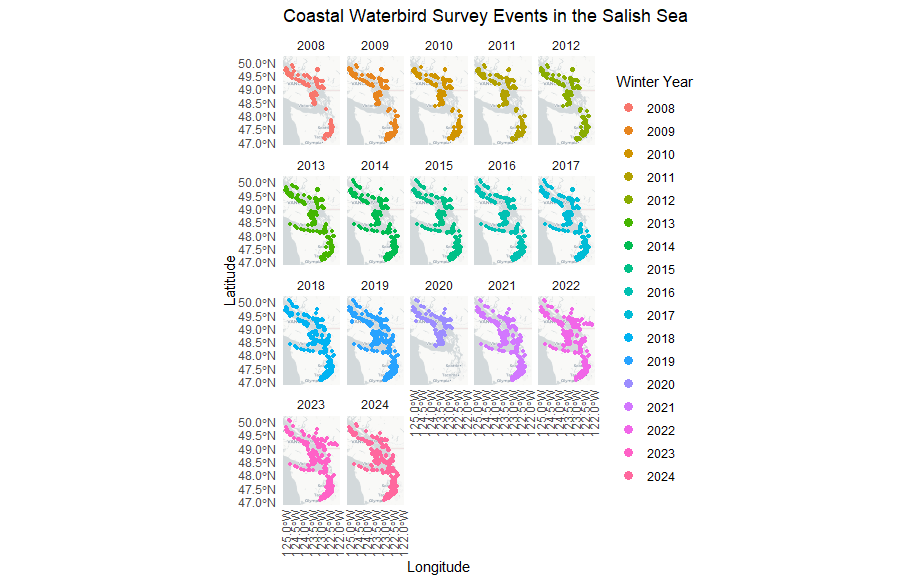
\includegraphics{Images/EventsMapbyYear.png}

}

\caption{Alt text for accessibility}

\end{figure}%

\bookmarksetup{startatroot}

\chapter{Analysis and Visualization}\label{analysis-and-visualization}

Run setup if starting a new environment. Load previously saved data and
format for analysis.

\begin{Shaded}
\begin{Highlighting}[]
\FunctionTok{source}\NormalTok{(}\StringTok{"Scripts/00\_Setup.R"}\NormalTok{)}

\CommentTok{\#Manually Specify the start and end year of the analysis. These years should match those selected for the data cleaning scripts. }
\NormalTok{Y1 }\OtherTok{=} \DecValTok{2008}
\NormalTok{Y2 }\OtherTok{=} \DecValTok{2024}

\CommentTok{\#Load your saved species data }
\NormalTok{sp.data}\OtherTok{\textless{}{-}}\FunctionTok{read.csv}\NormalTok{(}\StringTok{"Data/sp.data.csv"}\NormalTok{)}
\CommentTok{\#Load your saved events data which is needed for zero{-}filling}
\NormalTok{events}\OtherTok{\textless{}{-}}\FunctionTok{read.csv}\NormalTok{(}\StringTok{"Data/events.csv"}\NormalTok{)}

\CommentTok{\#Create a spatial points layers for graphing results}
\NormalTok{loc}\OtherTok{\textless{}{-}}\NormalTok{events }\SpecialCharTok{\%\textgreater{}\%} \FunctionTok{select}\NormalTok{(SurveyAreaIdentifier, DecimalLatitude, DecimalLongitude) }\SpecialCharTok{\%\textgreater{}\%} \FunctionTok{distinct}\NormalTok{()}
\NormalTok{xy}\OtherTok{\textless{}{-}}\FunctionTok{st\_as\_sf}\NormalTok{(loc, }\AttributeTok{coords =} \FunctionTok{c}\NormalTok{(}\StringTok{"DecimalLongitude"}\NormalTok{, }\StringTok{"DecimalLatitude"}\NormalTok{))}
\FunctionTok{st\_crs}\NormalTok{(xy)}\OtherTok{\textless{}{-}}\StringTok{"+proj=longlat +datum=NAD83"}

\CommentTok{\#Load the Salish Sea Water Polygon for graphing results }
\NormalTok{map}\OtherTok{\textless{}{-}} \FunctionTok{st\_read}\NormalTok{(}\StringTok{"Data/Spatial/Salish\_Sea\_Water\_Polygon.shp"}\NormalTok{)}

\CommentTok{\#ensure the coordinate reference systems are the same}
\NormalTok{mapCRS}\OtherTok{\textless{}{-}}\FunctionTok{st\_crs}\NormalTok{(map) }\CommentTok{\#get the CRS of the poly data}
\NormalTok{xy}\OtherTok{\textless{}{-}}\FunctionTok{st\_transform}\NormalTok{(xy, mapCRS) }\CommentTok{\#transform }
\end{Highlighting}
\end{Shaded}

\section{Set Analysis Parameters}\label{3.1Analysis}

Here the user has several customization options.

\subsection{Model Type}\label{3.1.1Analysis}

You can choose the continuous space ``SPDE'' or discrete space ``iCAR''
method.

\begin{Shaded}
\begin{Highlighting}[]
\CommentTok{\#model\textless{}{-}"iCAR"}
\NormalTok{model}\OtherTok{\textless{}{-}}\StringTok{"SPDE"}
\end{Highlighting}
\end{Shaded}

If doing an SPDE model, you may define your \texttt{area} as
``SalishSea'', ``BCCWS'', or ``PSSS''. Only sites with more than 10
years of data will be retained in the analysis.

\begin{Shaded}
\begin{Highlighting}[]
\ControlFlowTok{if}\NormalTok{(model }\SpecialCharTok{==} \StringTok{"SPDE"}\NormalTok{)\{}
\NormalTok{area }\OtherTok{\textless{}{-}} \StringTok{"SALISHSEA"} \CommentTok{\#one word to be compatible with the code.}
\CommentTok{\#area \textless{}{-} "BCCWS"}
\CommentTok{\#area \textless{}{-} "PSSS"}
\NormalTok{\}}
\end{Highlighting}
\end{Shaded}

If doing an iCAR model, upload the desired spatial polygon for the
analysis. We use ``Watersheds in the Salish Sea Bioregion'' layer from
the \href{https://salish-sea-atlas-data-wwu.hub.arcgis.com/}{Salish Sea
Atlas Data} as an example.

A polygon should have counts in all years to ensure that sampling is
complete and consistent. Those that have incomplete time series are
removed.

\begin{Shaded}
\begin{Highlighting}[]
\ControlFlowTok{if}\NormalTok{(model }\SpecialCharTok{==} \StringTok{"iCAR"}\NormalTok{)\{}
  
\NormalTok{  assignment\_method }\OtherTok{\textless{}{-}} \StringTok{"within"}  
\CommentTok{\# assignment\_method \textless{}{-} "nearest"}
  
\CommentTok{\# Load and prepare polygon}
\NormalTok{  poly }\OtherTok{\textless{}{-}} \FunctionTok{st\_read}\NormalTok{(}\StringTok{"Data/Spatial/Salish\_Sea\_Watersheds.shp"}\NormalTok{) }\SpecialCharTok{\%\textgreater{}\%} 
    \FunctionTok{st\_make\_valid}\NormalTok{() }\SpecialCharTok{\%\textgreater{}\%} 
    \FunctionTok{st\_transform}\NormalTok{(}\FunctionTok{st\_crs}\NormalTok{(mapCRS))  }\CommentTok{\# Ensure CRS matches points}
  
\CommentTok{\#List available fields for user selection}
  \FunctionTok{print}\NormalTok{(}\FunctionTok{names}\NormalTok{(poly))}

\CommentTok{\#Prompt user to select polygon ID and area fields}
\NormalTok{  polygon\_id\_field }\OtherTok{\textless{}{-}} \StringTok{"Name"} \CommentTok{\#Enter the field name for polygon ID (e.g., \textquotesingle{}WatershedID\textquotesingle{})}
\NormalTok{  area\_field }\OtherTok{\textless{}{-}} \StringTok{""} \CommentTok{\#Enter the field name for area (or leave blank if none or you desire equal weights)}

\CommentTok{\#Rename fields to \textquotesingle{}Name\textquotesingle{} and \textquotesingle{}Area\textquotesingle{}. If polygon area is missing, this will be created and assigned to 1. Analytically, this means the "Study Area" trend will be equally weighted across all polygons. }
\NormalTok{  poly }\OtherTok{\textless{}{-}}\NormalTok{ poly }\SpecialCharTok{\%\textgreater{}\%}
  \FunctionTok{rename}\NormalTok{(}\AttributeTok{Name =} \SpecialCharTok{!!}\NormalTok{polygon\_id\_field) }\SpecialCharTok{\%\textgreater{}\%}
  \FunctionTok{mutate}\NormalTok{(}\AttributeTok{Area =} \ControlFlowTok{if}\NormalTok{ (area\_field }\SpecialCharTok{!=} \StringTok{""}\NormalTok{) .data[[area\_field]] }\ControlFlowTok{else} \DecValTok{1}\NormalTok{)}
  
\CommentTok{\#Assignment method   }
 \ControlFlowTok{if}\NormalTok{ (assignment\_method }\SpecialCharTok{==} \StringTok{"within"}\NormalTok{) \{}
  \CommentTok{\# Assign points to polygons only if strictly within}
\NormalTok{  xy\_assigned }\OtherTok{\textless{}{-}} \FunctionTok{st\_join}\NormalTok{(xy, poly, }\AttributeTok{join =}\NormalTok{ st\_within)}
\NormalTok{\} }\ControlFlowTok{else} \ControlFlowTok{if}\NormalTok{ (assignment\_method }\SpecialCharTok{==} \StringTok{"nearest"}\NormalTok{) \{}
  \CommentTok{\# Assign each point to the nearest polygon}
\NormalTok{  nearest\_poly\_index }\OtherTok{\textless{}{-}} \FunctionTok{st\_nearest\_feature}\NormalTok{(xy, poly)}
\NormalTok{  xy\_assigned }\OtherTok{\textless{}{-}}\NormalTok{ xy}
\NormalTok{  xy\_assigned}\SpecialCharTok{$}\NormalTok{Name }\OtherTok{\textless{}{-}}\NormalTok{ poly}\SpecialCharTok{$}\NormalTok{Name[nearest\_poly\_index]}
\NormalTok{  xy\_assigned}\SpecialCharTok{$}\NormalTok{Area }\OtherTok{\textless{}{-}}\NormalTok{ poly}\SpecialCharTok{$}\NormalTok{Area[nearest\_poly\_index]}
\NormalTok{\} }\ControlFlowTok{else}\NormalTok{ \{}
  \FunctionTok{stop}\NormalTok{(}\StringTok{"Unknown assignment method."}\NormalTok{)}
\NormalTok{\}}

\CommentTok{\# Drop polygons with no assigned points}
\NormalTok{used\_names }\OtherTok{\textless{}{-}} \FunctionTok{unique}\NormalTok{(}\FunctionTok{na.omit}\NormalTok{(xy\_assigned}\SpecialCharTok{$}\NormalTok{Name))}
\NormalTok{poly }\OtherTok{\textless{}{-}}\NormalTok{ poly }\SpecialCharTok{\%\textgreater{}\%} \FunctionTok{filter}\NormalTok{(Name }\SpecialCharTok{\%in\%}\NormalTok{ used\_names)}


 \CommentTok{\# Create grid table}
\NormalTok{grid }\OtherTok{\textless{}{-}}\NormalTok{ xy\_assigned }\SpecialCharTok{\%\textgreater{}\%}
  \FunctionTok{st\_drop\_geometry}\NormalTok{() }\SpecialCharTok{\%\textgreater{}\%}
  \FunctionTok{filter}\NormalTok{(Name }\SpecialCharTok{\%in\%}\NormalTok{ poly}\SpecialCharTok{$}\NormalTok{Name) }\SpecialCharTok{\%\textgreater{}\%}
  \FunctionTok{select}\NormalTok{(SurveyAreaIdentifier, Name, Area) }\SpecialCharTok{\%\textgreater{}\%}
  \FunctionTok{distinct}\NormalTok{() }\SpecialCharTok{\%\textgreater{}\%}
  \FunctionTok{mutate}\NormalTok{(}\AttributeTok{alpha\_i =} \FunctionTok{as.integer}\NormalTok{(}\FunctionTok{factor}\NormalTok{(Name)))}

\CommentTok{\# Merge grid info back to events}
\NormalTok{events }\OtherTok{\textless{}{-}}\NormalTok{ events }\SpecialCharTok{\%\textgreater{}\%}
  \FunctionTok{left\_join}\NormalTok{(grid, }\AttributeTok{by =} \StringTok{"SurveyAreaIdentifier"}\NormalTok{) }\SpecialCharTok{\%\textgreater{}\%}
  \FunctionTok{drop\_na}\NormalTok{(Name)}

  \CommentTok{\# Visualization}
\NormalTok{  spatial\_plot }\OtherTok{\textless{}{-}} \FunctionTok{ggplot}\NormalTok{() }\SpecialCharTok{+}
    \FunctionTok{geom\_sf}\NormalTok{(}\AttributeTok{data =}\NormalTok{ poly, }\FunctionTok{aes}\NormalTok{(}\AttributeTok{fill =}\NormalTok{ Name), }\AttributeTok{color =} \StringTok{"black"}\NormalTok{) }\SpecialCharTok{+}
    \FunctionTok{geom\_sf}\NormalTok{(}\AttributeTok{data =}\NormalTok{ xy, }\AttributeTok{color =} \StringTok{"black"}\NormalTok{, }\AttributeTok{size =} \DecValTok{1}\NormalTok{) }\SpecialCharTok{+}
    \FunctionTok{theme\_minimal}\NormalTok{()}
  
  \FunctionTok{print}\NormalTok{(spatial\_plot)}
  \FunctionTok{ggsave}\NormalTok{(}\FunctionTok{file.path}\NormalTok{(plot.dir, }\StringTok{"iCAR\_Spatial\_Plot.jpeg"}\NormalTok{), }
         \AttributeTok{plot =}\NormalTok{ spatial\_plot, }\AttributeTok{width =} \DecValTok{8}\NormalTok{, }\AttributeTok{height =} \DecValTok{6}\NormalTok{, }\AttributeTok{dpi =} \DecValTok{300}\NormalTok{)}
\NormalTok{\}}
\end{Highlighting}
\end{Shaded}

\begin{figure}[H]

{\centering 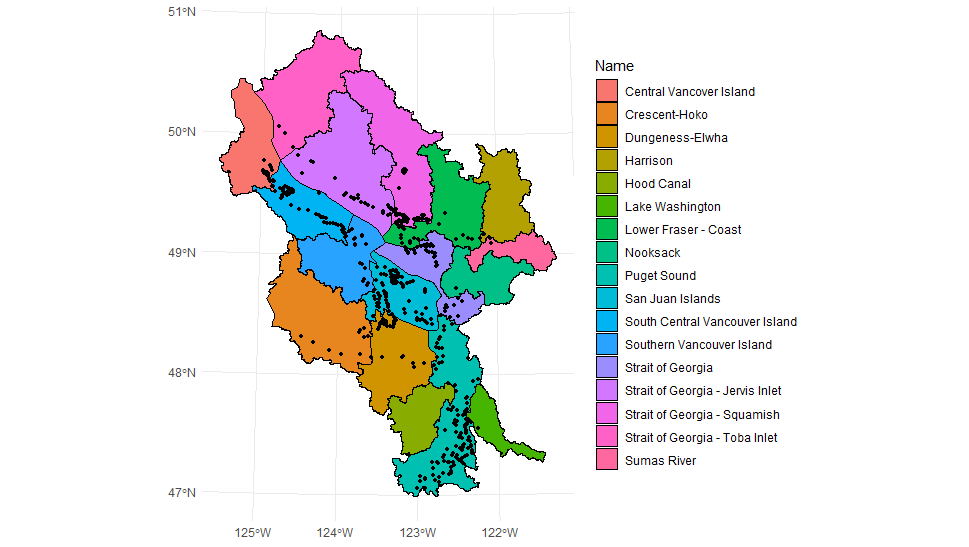
\includegraphics{Images/WatershedSampleMap.png}

}

\caption{Alt text for accessibility}

\end{figure}%

\subsection{Species or Guild Specific Analysis}\label{3.1.2Analysis}

For a species-specific analysis, select the species you wish to analyse.

\begin{Shaded}
\begin{Highlighting}[]
\CommentTok{\#To view your options of species}
\NormalTok{species}\OtherTok{\textless{}{-}}\FunctionTok{unique}\NormalTok{(sp.data}\SpecialCharTok{$}\NormalTok{CommonName)}
\CommentTok{\#view(species)}

\CommentTok{\#Create a list of species using all available species in the dataset.}
\NormalTok{species.list}\OtherTok{\textless{}{-}}\FunctionTok{tolower}\NormalTok{(}\StringTok{"All"}\NormalTok{) }\CommentTok{\#R is case sensitive}

\CommentTok{\#Or you can manually select species. Ensure case and spelling is correct. }
\CommentTok{\#species.list \textless{}{-} c("American Wigeon", "Common Loon", "Large Gull") }
\end{Highlighting}
\end{Shaded}

For a guild-specific analysis, change \texttt{guild} to ``Yes'' and
specify the \texttt{type} as either ``migration'', ``diet'', or
``family''. This will override the species list above.

\emph{You do not need to run this code chunk if doing a species-specific
analysis. Default guild is set to ``No'' in the setup script.}

\begin{Shaded}
\begin{Highlighting}[]
\NormalTok{guild }\OtherTok{\textless{}{-}} \StringTok{"yes"}

\CommentTok{\#To view your options of guilds}
\NormalTok{migration}\OtherTok{\textless{}{-}}\FunctionTok{unique}\NormalTok{(sp.data}\SpecialCharTok{$}\NormalTok{Migration)}
\CommentTok{\#view(migration)}

\NormalTok{diet}\OtherTok{\textless{}{-}}\FunctionTok{unique}\NormalTok{(sp.data}\SpecialCharTok{$}\NormalTok{Diet)}
\CommentTok{\#view(diet)}

\NormalTok{family}\OtherTok{\textless{}{-}}\FunctionTok{unique}\NormalTok{(sp.data}\SpecialCharTok{$}\NormalTok{family\_name)}
\CommentTok{\#view(family)}

\CommentTok{\#select on of the options for the analysis}
\NormalTok{type }\OtherTok{\textless{}{-}}\StringTok{"migration"}
\end{Highlighting}
\end{Shaded}

\subsection{Minimum Data Requirement}\label{3.1.3Analysis}

Select the minimum data requirements for the analysis. The ones selected
here were done following the inspection of the International dataset.
However, finer scale assessment may need to assess their suitability.

\begin{Shaded}
\begin{Highlighting}[]
\CommentTok{\#The minimum data required across sites with at least one detection:}

\NormalTok{min.abundance }\OtherTok{\textless{}{-}} \DecValTok{10} \CommentTok{\#Overall abundance per year \textgreater{} 10}
\NormalTok{min.years }\OtherTok{\textless{}{-}}\NormalTok{ (Y2}\SpecialCharTok{{-}}\NormalTok{Y1)}\SpecialCharTok{/}\DecValTok{2} \CommentTok{\#Detected in \textgreater{} one{-}half of the survey years}
\NormalTok{nsites }\OtherTok{\textless{}{-}} \DecValTok{10} \CommentTok{\#Detected at \textgreater{} 10 survey sites}
\end{Highlighting}
\end{Shaded}

\subsection{Model Specifications}\label{model-specifications}

Select the distributional family, and set random and spatial priors, or
retain the defaults. These priors were selected based on model
assessments for the full study area.

\begin{Shaded}
\begin{Highlighting}[]
\CommentTok{\#Here we select \textquotesingle{}nbinomal\textquotesingle{} but this may need to adjust if there is residual overdispersion. }

\NormalTok{fam}\OtherTok{\textless{}{-}}\StringTok{\textquotesingle{}nbinomial\textquotesingle{}}
\CommentTok{\#fam\textless{}{-}\textquotesingle{}poisson\textquotesingle{}}

\CommentTok{\#Priors for the random effects}
\NormalTok{hyper.iid }\OtherTok{\textless{}{-}} \FunctionTok{list}\NormalTok{(}\AttributeTok{prec =} \FunctionTok{list}\NormalTok{(}\AttributeTok{prior =} \StringTok{"pc.prec"}\NormalTok{, }\AttributeTok{param =} \FunctionTok{c}\NormalTok{(}\DecValTok{1}\NormalTok{, }\FloatTok{0.01}\NormalTok{)))}

\CommentTok{\#SPDE spatial priors used to make the model mesh}
\NormalTok{prior.range }\OtherTok{=} \FunctionTok{c}\NormalTok{(}\DecValTok{20}\NormalTok{, }\FloatTok{0.5}\NormalTok{)  }\CommentTok{\# 50\% probability range \textgreater{}20 km  }
\NormalTok{prior.sigma }\OtherTok{=} \FunctionTok{c}\NormalTok{(}\DecValTok{1}\NormalTok{, }\FloatTok{0.1}\NormalTok{)   }\CommentTok{\# 10\% probability stdev \textgreater{}1 }
\end{Highlighting}
\end{Shaded}

\begin{figure}[H]

{\centering 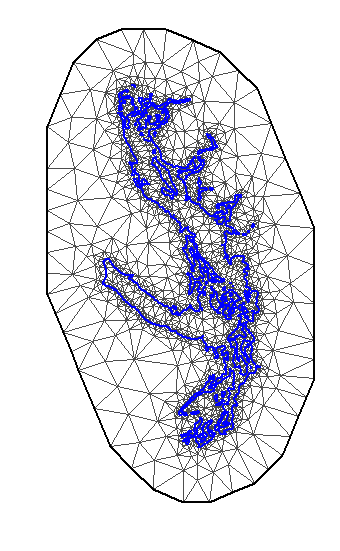
\includegraphics{Images/SPDEModelMesh.png}

}

\caption{Alt text for accessibility}

\end{figure}%

\section{Analysis}\label{3.2Analysis}

Create output tables to the \texttt{Output} folder using a custom file
\texttt{name}.

The files that this code creates is a file for Annual Indices for each
sampling site, end-point Trends, and a file with the Dispersion
statistic.

You are ready to start your analysis! The analysis will write results to
the files on the folder and also create some plots for model checking.

\begin{Shaded}
\begin{Highlighting}[]
\CommentTok{\#Give your analytically output file a unique name (e.g., BCCWS\_Species, SalishSea\_Migration, Watershed\_Species), }

\NormalTok{name}\OtherTok{\textless{}{-}}\StringTok{"SalishSea\_Species"}

\CommentTok{\#This is the template used for the State of Canada\textquotesingle{}s Birds and is required for upload into NatureCounts}

\CommentTok{\#Create output tables, which will include your custom name and the \textasciigrave{}model\textasciigrave{} you specified.}
\FunctionTok{output\_tables}\NormalTok{(name, model)}

\CommentTok{\#Now we can initiate the analysis based on the \textasciigrave{}model\textasciigrave{} you previously specified.   }
\FunctionTok{run\_analysis}\NormalTok{(model)}
\end{Highlighting}
\end{Shaded}

Note that the Dispersion Statistic file in the Output folder should be
reviewed after the analysis. If the statistic is \textgreater{} 10 you
should inspect the FitPlots in the Plot directory. In this case we will
want to rerun using a different distributional assumption on the counts.
This can be done by manually changing the \texttt{fam} to Poission and
selecting these species to be rerun.

\section{Results}\label{3.3Vis}

The analysis calculates trends using both the end point method and a
slope through the calculated annual indices of abundance. When mapping
the results, the user needs to select which \texttt{trend} outputs they
would like to view as either ``Endpoint'' or ``Slope''.

\begin{Shaded}
\begin{Highlighting}[]
\NormalTok{trend }\OtherTok{\textless{}{-}} \StringTok{"Slope"} 
\CommentTok{\#trend \textless{}{-} "Endpoint"}

\CommentTok{\#Graph your outputs}
\FunctionTok{graph\_results}\NormalTok{(model, name, trend)}
\end{Highlighting}
\end{Shaded}

Visually map trends per survey site resulting from the SPDE analysis.

\begin{Shaded}
\begin{Highlighting}[]
\NormalTok{\#| standalone: true}

\NormalTok{\# {-}{-}{-} 1. Load your data (replace file names as needed) {-}{-}{-}}
\NormalTok{trends \textless{}{-} read.csv(file.path(out.dir, paste0(name, "\_TrendsSlope\_SPDE.csv"))) \%\textgreater{}\% }
\NormalTok{  drop\_na(results\_code) \%\textgreater{}\% }
\NormalTok{  select(area\_code, species\_code, trnd, lower\_ci, upper\_ci, percent\_change)}

\NormalTok{events \textless{}{-} read\_csv("Data/events.csv")}
\NormalTok{events \textless{}{-} events \%\textgreater{}\% select(SurveyAreaIdentifier, wyear, DecimalLatitude, DecimalLongitude) \%\textgreater{}\% distinct()}

\NormalTok{annual\_indices \textless{}{-} read.csv(file.path(out.dir, paste0(name, "\_AnnualIndices\_SPDE.csv"))) \%\textgreater{}\% }
\NormalTok{  drop\_na(results\_code) }

\NormalTok{\# {-}{-}{-} 2. Merge trends with site coordinates {-}{-}{-}}
\NormalTok{trends\_map \textless{}{-} trends \%\textgreater{}\%}
\NormalTok{  left\_join(events, by = c("area\_code" = "SurveyAreaIdentifier"))}

\NormalTok{\# {-}{-}{-} 3. Prepare popup content (basic version) {-}{-}{-}}
\NormalTok{trends\_map \textless{}{-} trends\_map \%\textgreater{}\%}
\NormalTok{  mutate(}
\NormalTok{    popup = paste0(}
\NormalTok{      "\textless{}b\textgreater{}Area:\textless{}/b\textgreater{} ", area\_code, "\textless{}br\textgreater{}",}
\NormalTok{      "\textless{}b\textgreater{}Species:\textless{}/b\textgreater{} ", species\_code, "\textless{}br\textgreater{}",}
\NormalTok{      "\textless{}b\textgreater{}Trend (slope):\textless{}/b\textgreater{} ", round(trnd, 2), "\textless{}br\textgreater{}",}
\NormalTok{      "\textless{}b\textgreater{}95\% CI:\textless{}/b\textgreater{} [", round(lower\_ci, 2), ", ", round(upper\_ci, 2), "]\textless{}br\textgreater{}",}
\NormalTok{      "\textless{}b\textgreater{}Percent Change:\textless{}/b\textgreater{} ", round(percent\_change, 1), "\%\textless{}br\textgreater{}"}
\NormalTok{      \# Optionally, add more info or links here}
\NormalTok{    )}
\NormalTok{  )}

\NormalTok{\# {-}{-}{-} 4. Set color palette for trend slope {-}{-}{-}}
\NormalTok{pal \textless{}{-} colorNumeric(palette = "RdYlBu", domain = trends\_map$trnd, reverse = TRUE)}

\NormalTok{\# {-}{-}{-} 5. Build and display the Leaflet map {-}{-}{-}}
\NormalTok{leaflet(trends\_map) \%\textgreater{}\%}
\NormalTok{  addProviderTiles("CartoDB.Positron") \%\textgreater{}\%}
\NormalTok{  addCircleMarkers(}
\NormalTok{    lng = \textasciitilde{}DecimalLongitude,}
\NormalTok{    lat = \textasciitilde{}DecimalLatitude,}
\NormalTok{    radius = 8,}
\NormalTok{    color = \textasciitilde{}pal(trnd),}
\NormalTok{    stroke = TRUE,}
\NormalTok{    fillOpacity = 0.8,}
\NormalTok{    popup = \textasciitilde{}popup}
\NormalTok{  ) \%\textgreater{}\%}
\NormalTok{  addLegend(}
\NormalTok{    "bottomright",}
\NormalTok{    pal = pal,}
\NormalTok{    values = \textasciitilde{}trnd,}
\NormalTok{    title = "Trend (slope)",}
\NormalTok{    opacity = 1}
\NormalTok{  )}
\NormalTok{shinyApp(ui, server)}
\end{Highlighting}
\end{Shaded}

\begin{Shaded}
\begin{Highlighting}[]
\NormalTok{\#| standalone: true}

\NormalTok{ui \textless{}{-} fluidPage(}
\NormalTok{  titlePanel("Species Trends Map"),}
\NormalTok{  leafletOutput("map", height = 600)}
\NormalTok{)}

\NormalTok{server \textless{}{-} function(input, output, session) \{}
\NormalTok{  trends \textless{}{-} read.csv(file.path(out.dir, paste0(name, "\_TrendsSlope\_SPDE.csv"))) \%\textgreater{}\% }
\NormalTok{  drop\_na(results\_code) \%\textgreater{}\% }
\NormalTok{  select(area\_code, species\_code, trnd, lower\_ci, upper\_ci, percent\_change)}

\NormalTok{events \textless{}{-} read\_csv("Data/events.csv")}
\NormalTok{events \textless{}{-} events \%\textgreater{}\% select(SurveyAreaIdentifier, wyear, DecimalLatitude, DecimalLongitude) \%\textgreater{}\% distinct()}

\NormalTok{annual\_indices \textless{}{-} read.csv(file.path(out.dir, paste0(name, "\_AnnualIndices\_SPDE.csv"))) \%\textgreater{}\% }
\NormalTok{  drop\_na(results\_code) }

\NormalTok{\# {-}{-}{-} 2. Merge trends with site coordinates {-}{-}{-}}
\NormalTok{trends\_map \textless{}{-} trends \%\textgreater{}\%}
\NormalTok{  left\_join(events, by = c("area\_code" = "SurveyAreaIdentifier"))}

\NormalTok{\# {-}{-}{-} 3. Prepare popup content (basic version) {-}{-}{-}}
\NormalTok{trends\_map \textless{}{-} trends\_map \%\textgreater{}\%}
\NormalTok{  mutate(}
\NormalTok{    popup = paste0(}
\NormalTok{      "\textless{}b\textgreater{}Area:\textless{}/b\textgreater{} ", area\_code, "\textless{}br\textgreater{}",}
\NormalTok{      "\textless{}b\textgreater{}Species:\textless{}/b\textgreater{} ", species\_code, "\textless{}br\textgreater{}",}
\NormalTok{      "\textless{}b\textgreater{}Trend (slope):\textless{}/b\textgreater{} ", round(trnd, 2), "\textless{}br\textgreater{}",}
\NormalTok{      "\textless{}b\textgreater{}95\% CI:\textless{}/b\textgreater{} [", round(lower\_ci, 2), ", ", round(upper\_ci, 2), "]\textless{}br\textgreater{}",}
\NormalTok{      "\textless{}b\textgreater{}Percent Change:\textless{}/b\textgreater{} ", round(percent\_change, 1), "\%\textless{}br\textgreater{}"}
\NormalTok{      \# Optionally, add more info or links here}
\NormalTok{    )}
\NormalTok{  )}

\NormalTok{  pal \textless{}{-} colorNumeric(palette = "RdYlBu", domain = trends\_map$trnd, reverse = TRUE)}
  
\NormalTok{  output$map \textless{}{-} renderLeaflet(\{}
\NormalTok{    leaflet(trends\_map) \%\textgreater{}\%}
\NormalTok{      addProviderTiles("CartoDB.Positron") \%\textgreater{}\%}
\NormalTok{      addCircleMarkers(}
\NormalTok{        lng = \textasciitilde{}DecimalLongitude,}
\NormalTok{        lat = \textasciitilde{}DecimalLatitude,}
\NormalTok{        radius = 8,}
\NormalTok{        color = \textasciitilde{}pal(trnd),}
\NormalTok{        stroke = TRUE,}
\NormalTok{        fillOpacity = 0.8,}
\NormalTok{        popup = \textasciitilde{}popup}
\NormalTok{      ) \%\textgreater{}\%}
\NormalTok{      addLegend(}
\NormalTok{        "bottomright",}
\NormalTok{        pal = pal,}
\NormalTok{        values = \textasciitilde{}trnd,}
\NormalTok{        title = "Trend (slope)",}
\NormalTok{        opacity = 1}
\NormalTok{      )}
\NormalTok{  \})}
\NormalTok{\}}

\NormalTok{shinyApp(ui, server)}
\end{Highlighting}
\end{Shaded}

\bookmarksetup{startatroot}

\chapter{Resources}\label{resources}

\section{Birds Canada GitHub}\label{9.9BirdsCan}

All R scripts and resources associated with this project, as well as
many other tools and tutorials, are available on the
\href{https://github.com/BirdsCanada}{Birds Canada GitHub} page.

\begin{figure}[H]

{\centering 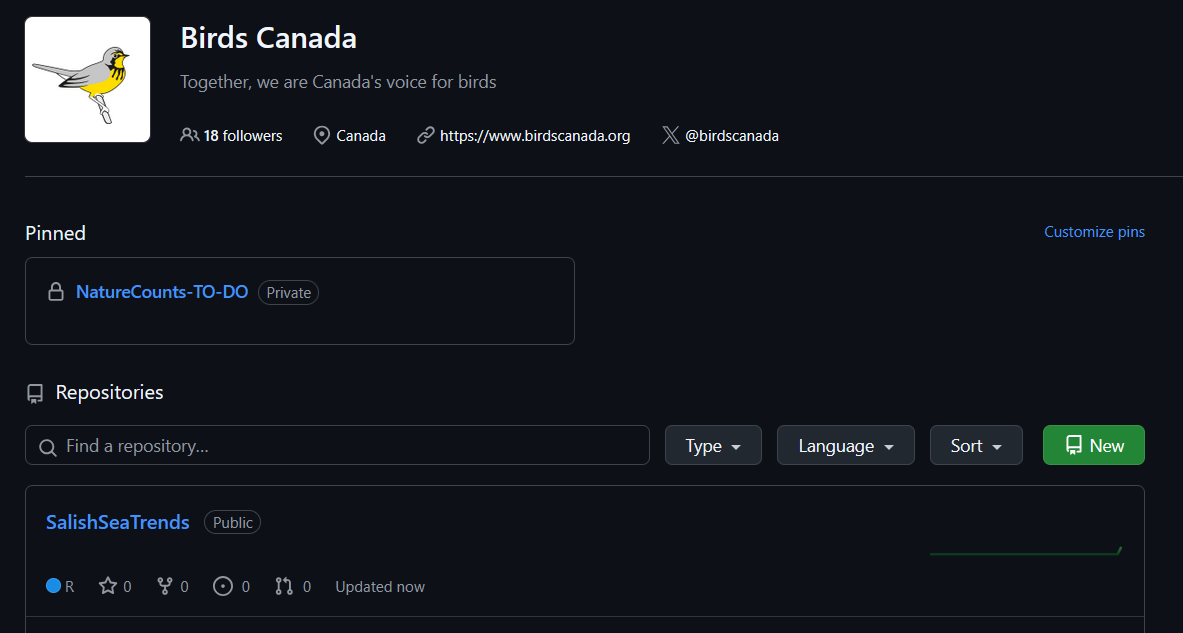
\includegraphics{Images/BirdsCanadaGithub.png}

}

\caption{Alt text for accessibility}

\end{figure}%

This repository is regularly updated and serves as the central hub for
sharing code related to Birds Canada's monitoring and research programs.
If you run into issues using this code, or it generates errors, please
open a git issue of email dethier@birdscanada.org.

To access the code visit: https://github.com/BirdsCanada/SalishSeaTrends

You can view files directly on GitHub, or download individual scripts
and entire repositories by clicking the green Code button and selecting
Download ZIP.For advanced users, you can clone repositories using Git
into RStudio using the following command in the Terminal:

git clone https://github.com/BirdsCanada/SalishSeaTrends.git

For tutorials and additional resources on using the NatureCounts R
package, see the
\href{https://birdscanada.github.io/naturecounts/articles/index.html}{NatureCounts
package website}.

If you are new to GitHub, Birds Canada also provides a
\href{https://birdscanada.github.io/BirdsCanada_GitHubGuide/}{Beginner's
Guide to GitHub} with step-by-step instructions for accessing and
sharing code.

Data users are encourage to review the
\href{https://birdscanada.github.io/TransboundaryData_SalishSea/}{Transboundary
avian data for the Salish Sea} user guide, which details addition avian
datasets and spatial data layers available for the Salish Sea.

\section{Downloadable R Scripts}\label{9.91BirdsCan}

\begin{itemize}
\tightlist
\item
  \href{Scripts/00_Setup.R}{00\_Setup.R}
\item
  \href{Scripts/Analysis_iCAR.R}{Analysis\_iCAR.R}
\item
  \href{Scripts/Analysis_SPDE.R}{Analysis\_SPDE.R}
\item
  \href{Scripts/BCCWSClean.R}{BCCWSClean.R}
\item
  \href{Scripts/PSSSClean.R}{PSSSClean.R}
\item
  \href{Scripts/Graph_iCAR.R}{Graph\_iCAR.R}
\item
  \href{Scripts/Graph_SPDE.R}{Graph\_SPDE.R}
\item
  \href{Scripts/OutputTables.R}{OutputTables.R}
\item
  \href{Scripts/PSSSBMDE.R}{PSSSBMDE.R}
\end{itemize}

\section{Downloadable Data}\label{9.92BirdsCan}

\begin{itemize}
\tightlist
\item
  \href{Data/GuildList.csv}{GuildList.csv}
\item
  \href{Data/Spatial/Salish_Sea_Water_Polygon.dbf}{Salish\_Sea\_Water\_Polygon.dbf}
\item
  \href{Data/Spatial/Salish_Sea_Water_Polygon.prj}{Salish\_Sea\_Water\_Polygon.prj}
\item
  \href{Data/Spatial/Salish_Sea_Water_Polygon.shp}{Salish\_Sea\_Water\_Polygon.shp}
\item
  \href{Data/Spatial/Salish_Sea_Water_Polygon.shx}{Salish\_Sea\_Water\_Polygon.shx}
\item
  \href{Data/Spatial/Salish_Sea_Watershed.dbf}{Salish\_Sea\_Watershed.dbf}
\item
  \href{Data/Spatial/Salish_Sea_Watershed.prj}{Salish\_Sea\_Watershed.prj}
\item
  \href{Data/Spatial/Salish_Sea_Watershed.shp}{Salish\_Sea\_Watershed.shp}
\item
  \href{Data/Spatial/Salish_Sea_Watershed.shx}{Salish\_Sea\_Watershed.shx}
\end{itemize}




\end{document}
